
\documentclass[12pt]{article}
\usepackage{geometry} % see geometry.pdf on how to lay out the page. There's lots.
\geometry{a4paper} % or letter or a5paper or ... etc
% \geometry{landscape} % rotated page geometry
\usepackage[parfill]{parskip}
% See the ``Article customise'' template for come common customisations
\usepackage{amsmath}
\usepackage{graphicx}
\title{Slides02}

%%% BEGIN DOCUMENT
\begin{document}

\maketitle
\tableofcontents
\newpage

\section{Computational Security}
We would like to have perfectly secret encryption. But $\prod:=<Gen,Enc,Dec>$ is not perfectly secret encryption scheme with $|\mathcal{K}| < |\mathcal{M}|$.
What can we expect from imperfect security?
\begin{itemize}
\item Replace impossibility (of perfectly secret encryption) by infeasibility
\item Practical scheme "emulating" perfect scheme for practical purposes 
\end{itemize}
\emph{Emulating?}\\
\textbf{Experiment} $Priv_{\mathcal{A},\prod}^{eav'}$

\begin{enumerate}
\item $\mathcal{A}$ \emph{not unbounded} outputs $m_0,m_1 \in \mathcal{M}$
\item Choose $k \leftarrow \mathcal{K}$ and  $b \leftarrow \{0,1\}$ and send $Enc_k(m_b)$ to $\mathcal{A}$
 \item $\mathcal{A}$ outputs $b'$
 \item Define $Priv_{\mathcal{A},\prod}^{eav}:=1$ iff $b=b'$
\end{enumerate}
\begin{equation}
Pr[Priv_{\mathcal{A},\prod}^{eav}:=1] = \frac{1}{2}+ \emph{ negligible term}
\end{equation}
\subsection{Concrete bounds}
Two relaxations:
\begin{enumerate}
\item $\mathcal{A}$ does not have unbounded power
	\begin{itemize}
	\item $10^9$ keys/sec
	\item $10^6$ computers
	\item $10^9$  seconds $\approx$ 30 years\\
	$=>$ makes $2^{80}$ steps
	\end{itemize}
\item $\mathcal{A}$ can have a small success probability
	\begin{itemize}
	\item Say $2^{-48}$, event with $Pr\approx 2^{-30}/sec$ occurs $<1/100$ years
	\end{itemize}
\end{enumerate}
Suggests that $|\mathcal{K}| = 2^{128}$ would be very nice.\\
Proposed solution:
\begin{itemize}
\item Design schemes that are $(t, \epsilon)$-secure
\end{itemize}
Which gives concrete bounds: We know what we can hold.
\newpage
\subsection{Asymptotic bounds}
Concrete security bounds:
\begin{itemize}
\item Suppose $<Gen,Enc,Dec>$ is  $(t, \epsilon)$-secure, what about 5t?
\item How does  $(t, \epsilon)$ change with key size?\\
Can encryption cost become $>$ cryptanalysis cost?
\end{itemize}
Another solution:
\begin{itemize}
\item  Consider $(t, \epsilon)$ as a function of a security parameter n (e.g., length of the key)
\item Define a class of "feasible" algorithms\\
Number of steps as a function of n, f(n)
\item Show that: $\forall$ feasible strategy of $\mathcal{A}$, $Pr[\mathcal{A}\,wins ] \rightarrow 0$, goes to 0 fast when n increases
\end{itemize}
$\prod$ is secure if:
\begin{itemize}
\item every "feasible" adversary strategy succeeds with "negligible" probability as a function of the security parameter
\end{itemize}
\subsection{Feasible strategy / Efficient algorithm}
Let n be the length of the numbers\\
Simple computational problems:
\begin{itemize}
\item Addition: $\mathcal{O}(n)$
\item Multiplication: $\mathcal{O}(n^2)$
\item (Modular) Exponentiation: $\mathcal{O}(n^3)$
\item Search in ordered list: $\mathcal{O}(log(n))$
\end{itemize}
Computationally hard problems:
\begin{itemize}
\item Integer factorization: $2^{\mathcal{O}(\sqrt{n*log(n)})}$
\item Exhaustive key search: $\mathcal{O}(2^n)$
\end{itemize}
\newpage
Polynomial-time algorithms are efficient:
\begin{itemize}
\item $\mathcal{A}$ is efficient if $\exists$ polynomial $p$ s.t.
\item $\mathcal{A}$ takes $\le$ $p(|x|)$ steps
\end{itemize}
Is a probabilistic $\mathcal{A}$ more powerful?\\
\emph{Efficient $\iff$ Probabilistic polynomial-time (PPT)}
\begin{itemize}
\item $\mathcal{A}$ is efficient if $\exists$ polynomial $p$ s.t.
\item $\mathcal{A}$ takes $\le$ $p(|x|)$ steps, which include tossing a coin (randomness)
\end{itemize}
\subsection{Negligible functions}
\emph{Negligible:} Decreases faster than any inverse polynomial.\\
$f$ is negligible iff:\\
$\forall$ positive polynomial $p$, $\exists$N such that $\forall n\ge N$:\\
\begin{equation}
f(n) \le \frac{1}{p(n)}
\end{equation}
Examples: $2^{-n}$, $n^{-log(n)}$

\subsection{Asymptotic security}
\begin{itemize}
\item Tells us how primitives behave
\item PPT algorithms and negligible functions are convenient to use
	\begin{itemize}
	\item PPT algo running a PPT algo is still PPT
	\item f negl. and p poly. $\rightarrow$ p*f negl.
	\end{itemize}
\end{itemize}
\newpage
\section{Encryption}
What is encryption in a computational world?\\
A triple $<Gen,Enc,Dec>$ of PPT algorithms:
\begin{itemize}
\item $Gen$ probabilistically selects $k \leftarrow Gen(1^n)$
\item $Enc$ provides $c \leftarrow Enc_k(m)$
\item $Dec$ provides $m:=Dec_k(c)$
\end{itemize}
Correctness:
\begin{itemize}
\item $\forall$n, $k \leftarrow Gen(1^n)$, and $\forall m$:  $m:=Dec_k(Enc_k(m)) = m$
\end{itemize}
\subsection{Security for encryption }
\textbf{Experiment} $Priv_{\mathcal{A},\prod}^{eav}(n)$

\begin{enumerate}
\item $\mathcal{A}(1^n)$ outputs $m_0,m_1$ of identical lengths
\item pick $k \leftarrow Gen(1^n)$ and  $b \leftarrow \{0,1\}$ and send $c \leftarrow Enc_k(m_b)$ to $\mathcal{A}$
 \item $\mathcal{A}(c)$ outputs $b'$
 \item Define $Priv_{\mathcal{A},\prod}^{eav}(n):=1$ iff $b=b'$
\end{enumerate}
$\prod:=<Gen,Enc,Dec>$ has \emph{indistinguishable} encryptions in the presence of eavesdroppers if $\forall$ PPT $\mathcal{A}$, $\exists$ negl. $\epsilon$:
\begin{equation}
Pr[Priv_{\mathcal{A},\prod}^{eav}(n)=1] = \frac{1}{2} + \epsilon(n)
\end{equation}
\textbf{Efficiency and security depends on the security parameter.}

\subsubsection{Building secure encryption schemes}
Emulating a one-time pad, for $n < l(n)$
\begin{itemize}
\item $Gen(1^n)$: pick $k\leftarrow \{0,1\}^{l(n)}$, set $\mathcal{M} = \{0,1\}^{l(n)}$\\
$\rightarrow$ we want $ |k| < |m| = l(n)$, for any $m \in \mathcal{M}$\\
$\rightarrow $ Expand, $k \in \{0,1\}^n$ to $G(k) \in \{0,1\}^{l(n)}$
\item $Enc_k(m):$ Compute and return $c=m \oplus k$\\
$\rightarrow$ Instead, compute $c=m\oplus G(k)$\\
$\rightarrow$ Enough if G(k) is \emph{indistinguishable} of random
\item $Dec_k(c)$: Compute and return $m=c\oplus k$\\
$\rightarrow$ Instead, compute $c\oplus G(k)$
\end{itemize}
$G$ is called a \emph{pseudorandom} generator
\section{Pseudorandomness}
A deterministic poly-time algorithm $G$ is a pseudorandom generator (PRG) only if, for any n,\\
\begin{itemize}
\item $\forall s \in \{0,1\}^n, G(s) \in \{0,1\}^{l(n)}$ and $l(n) > n$
\item $\forall$ PPT $D$, $\exists$ negligible function $\epsilon$ s.t.
\begin{equation}
|Pr[D(r)=1]-Pr[D(G(s))=1]| \le \epsilon(n)
\end{equation}
Where $r\leftarrow \{0,1\}^{l(n)}$ and $s\leftarrow \{0,1\}^n$\\
$s$ is called the seed, and funciton $l$ us called the expansion factor of $G$.
\end{itemize}

Pseudorandom generators:
\begin{itemize}
\item Can only be computationally secure: $l(n) = 2*n$
\item $n$ should be large enough to avoid brute-force
\end{itemize}
\textbf{Pseudorandom generators exist iff one-way functions exist} \\
Existence of one-way functions $\rightarrow P \neq NP$\\
$\rightarrow$\textbf{Assumption: Pseudorandom generators exist}
\begin{center}
\begin{align*}
\text{Definition} & \Rightarrow \text{Assumption} \Rightarrow \text{Reduction}
\end{align*}
\end{center}

\emph{Theorem}:\\
If $G$ is a PRG, then $\prod$ is a (fixed length) encryption scheme that has indistinguishable encryption in the presence of an eavesdropper.\\
\emph{Proof}:
\begin{itemize}
\item $\forall$ PPT $\mathcal{A}$ with $\eta$ advantage
\item $\exists$ PPT $D$ for $G$ with $\eta$ advantage
\end{itemize}
Therefore, $\eta$ must be negligible.
\newpage
\subsection{Reduction}
Suppose:
\begin{equation}
Pr[Priv_{\mathcal{A},\prod}^{eav}(n)=1] = \frac{1}{2} + \eta(n)
\end{equation}
\begin{figure}[ht]
    \centering
    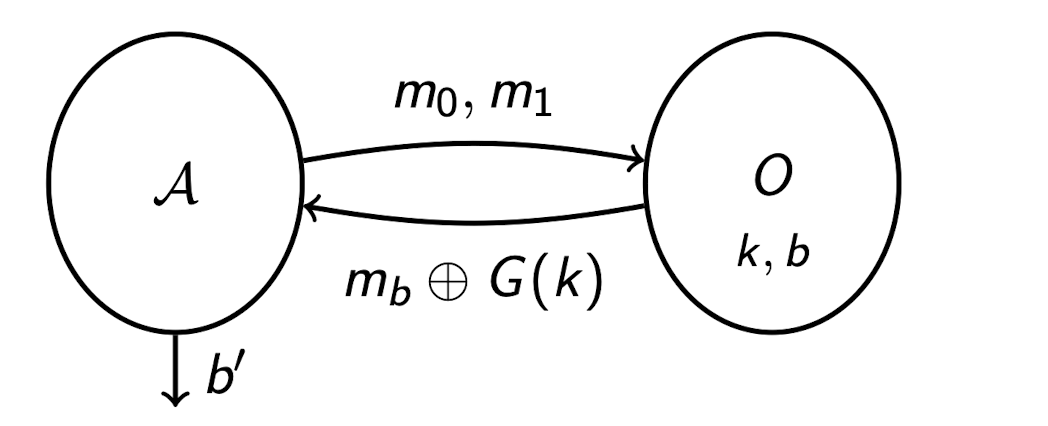
\includegraphics[width=8cm]{figures/f1.png}
    \caption{Reduction 1}
\end{figure}

$\rightarrow \mathcal{A}$ is s.t. $Pr[b=b']=  \frac{1}{2} + \eta(n)$ 

\begin{figure}[ht]
    \centering
    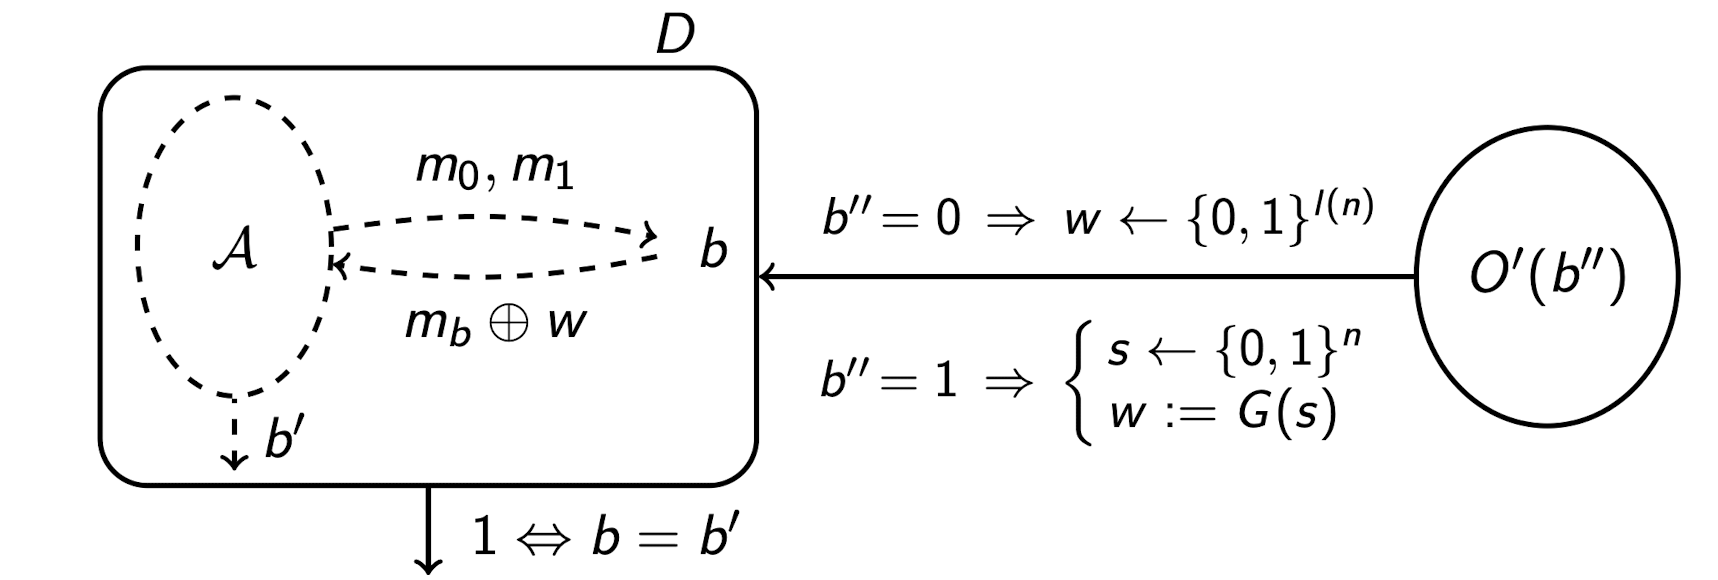
\includegraphics[width=12cm]{figures/f2.png}
    \caption{Reduction 2}
\end{figure}

Observe:
\begin{itemize}
\item If $b'' = 0$, Pr[$D$ outputs 1] = $\frac{1}{2}$ $\rightarrow$ one-time pad
\item If $b'' = 1$, Pr[$D$ outputs 1] = $\frac{1}{2} + \eta(n)$ $\rightarrow$ $Priv_{\mathcal{A},\prod}^{eav}(n)$\\
This means, when  $b'' = 1$, $D$ distinguishes with advantage $\eta(n)$
\item If $\mathcal{A}$ is PPT, then $D$ is PPT too
\end{itemize}
\newpage
Results:
\begin{itemize}
\item Encryption with keys shorted than messages
\item Proof is conditional, by reduction
\item Proof holds for computationally bounded adversaries, and leaves some probability of attack
\end{itemize}
\subsection{Variable-length encryption}
$\prod$ is restricted to messages with $|m| \le l(|k|)$
\begin{itemize}
\item We need $G$ with variable-length output
\item Use $G$ repeatedly until output is long enough
\item Preserves security if G is used poly many times
\end{itemize}
\section{Conclusion}
\begin{itemize}
\item Computational security opens doors for cryptography with shorter keys\\
We can encrypt $m$ of length $p(|k|)$
\item However, encrypting multiple message with the same key, it becomes insecure (even one-time pad)
\end{itemize}










































\end{document}